\documentclass{beamer}
\usetheme[color=ACMblue]{ACMNew}
\usepackage{beamernotes}
\usepackage{algpseudocodex}
\usepackage{lipsum}
\usepackage{minted}
\usemintedstyle{manni}
\pdfcompresslevel=9
\pdfobjcompresslevel=3

\title[ACM fun]{CS 438 Final Review}
\author{ACM @ UIUC}
%\institute{The Mental Institute}
\date{September 26, 2024}

\begin{document}

\begin{frame}
  \titlepage
\end{frame}
\bnote{This generates notes for pdfpc. These notes also appear
  on the handout/article versions.}

\begin{frame}[t]{Disclaimers and Logistics}
  \begin{itemize}
  \item \alert{Disclaimer:} We have not seen the exam. We have no idea what the questions are. However, we've taken the course and reviewed material/practice exams, so we have \alert{suspicions} as to what the questions will be like.
  \item This review session is being recorded. Recordings and slides will be distributed on Piazza and the ACM site at the end.
  \item \alert{Agenda:} We'll review all topics likely to be covered, working through some examples that may look like exam questions as we go, then review individual topics by request.
  \begin{itemize}
      \item Questions are designed to be written in the same style as previous exams but to be \textit{slightly} harder, so don't worry if you don't get everything right away!
  \end{itemize}
  \item We're just planning to cover second-half material, but have slides for the entire course- please let us know what you want to cover
  \item Please let us know if we're going too fast/slow, not speaking loud enough/speaking too loud, etc.
  \item If you have a question anytime during the review session, please ask! Someone else almost surely has a similar question.
  \item We'll provide a feedback form at the end of the session.
  \end{itemize}
\end{frame}

\begin{frame}
\frametitle{Table of Contents}
\tableofcontents
\end{frame}

\section{Foundations}

\begin{frame}[t]{Foundations I: Resource Sharing}
 \begin{itemize}
     \item A \alert{network} is just a set of \alert{elements} (servers, routers, etc.) connected together, that implements a set of \alert{protocols} for the purpose of \alert{sharing resources} at the end hosts
     \begin{itemize}
        \item Visualized as graph with elements as nodes and \alert{links} as the edges connecting them
        \item \pause Only one goal- deliver the data between edge nodes
     \end{itemize}
     \item \pause \alert{Statistical Multiplexing}: combining demands to share resources without overbuilding capacity, as aggregate of peak demand is much bigger than peak of aggregate demand. Two approaches:
    \begin{itemize}
        \item \pause \alert{Reservations/Circuit Switching}: Source sends call request, path between source and destination reserved + blocked off, communication happens, then circuit teardown. Used in some telephone + ATM protocols. Can share a channel using FDM (split frequencies) or TDM (round-robin whole resource)
        \item \pause \alert{Packets/Datagrams}: Packets contain data (body) + information on how/where to send it and where it came from (headers). No underutilization/blocked connections/setup costs and can route around link failures, but no guarantees on availiability/delay, and overhead from headers. Used basically everywhere. 
    \end{itemize}
 \end{itemize}    
\end{frame}
\begin{frame}[t]{Foundations II: Internet as IPC}
    \begin{itemize}
        \item Main problem: \alert{inter-process communication}, where processes may not be on the same machine
        \begin{exampleblock}{End-To-End Story}
            \begin{itemize}
                \item \pause Program opens \alert{socket} which allows it to connect to \alert{network stack}
                \item \pause \alert{DNS} maps name of target to \alert{address}
                \item \pause Network stack embeds address and \alert{port} of source/destination in datagram headers
                \item \pause \alert{Routers} create \alert{routing tables} to decide which \alert{outgoing link} to send packets along (knowing only local information). When link is free, forward packet to next router
                \item \pause When packet arrives at destination, forward to correct application
            \end{itemize}
        \end{exampleblock}
        \item Goal: Nodes shouldn't have to worry about the implementation details of other nodes, just the correct decision locally (modularity)
    \end{itemize}
\end{frame}

\begin{frame}[t]{Foundations III: Layering}
    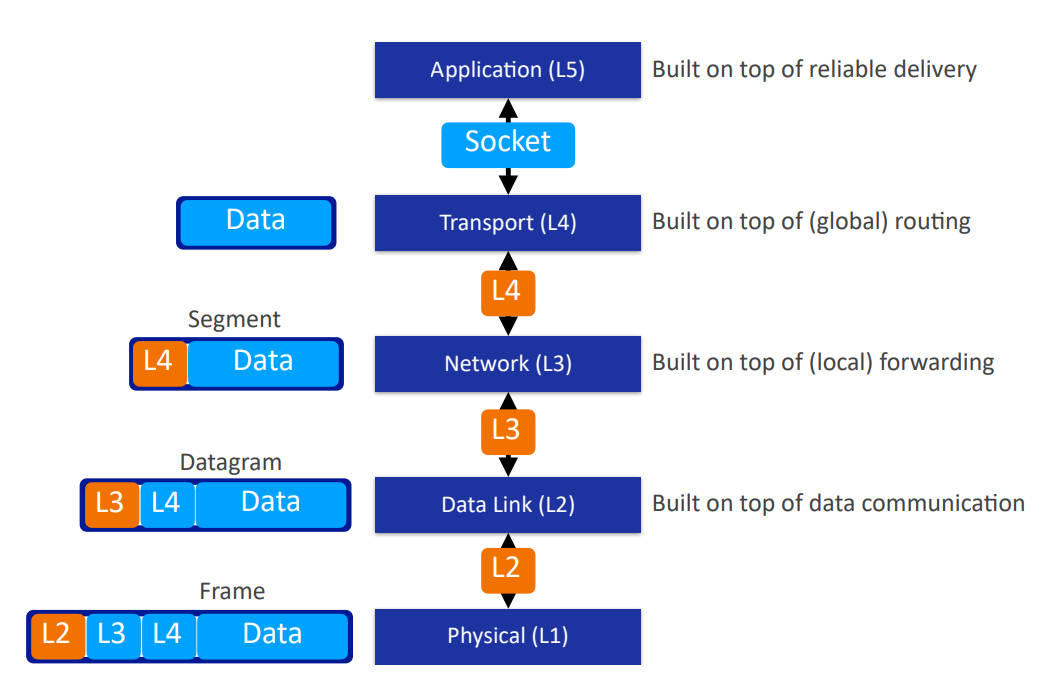
\includegraphics[height=12cm]{layer diagram.png}
\end{frame}

\begin{frame}[t]{Foundations IV: Desiderata}
    \begin{itemize}
        \item \alert{Data Loss}: some applications (video/audio) can tolerate it, others (file transfer/ssh/etc.) can't
        \begin{itemize}
            \item \pause \alert{Packet Error Rate} = $\frac{N}{P}$ for $N$ unrecoverable bit errors for $P$ packets. Packets can be recovered through error-correcting coding, depending on schema. 
            \item \pause Example: if bit error rate is $10^{-6}$, packet 10kb, no ECC, then PER is $1-(1-10^{-6})^{10240} = 1.0\%$
        \end{itemize}
        \item \pause \alert{Bandwidth}: some applications (video streaming) require some amount to be effective, but ``elastic apps'' can use whatever bandwidth they get
        \begin{itemize}
            \item \pause \alert{Throughput}: Number of \textit{total} correctly delivered bits in unit time
            \item \pause \alert{Goodput}: Number of \textit{application-layer} correctly delivered bits in unit time
        \end{itemize}
        \item \pause \alert{Timing}: some applications need packets to be delivered right away (video games/live conferencing/etc.). \alert{Per Packet Latency} = Transmit time + Propagation delay + Process time + Queuing Delay. Assuming packet length $L$, transmit rate $R$ bps
        \begin{itemize}
            \item \pause \alert{Transmit Time}: Time used by transmitter to write packet to wire ($\frac{L}{R}$)
            \item \pause \alert{Propagation Delay}: Time for packet to travel from transmitter to receiver ($\frac{\text{distance}}{\text{velocity}}$)
            \item \pause \alert{Process Time}: Time required for router to read header + decide route
            \item \pause \alert{Queuing Delay}: Time that a packet waits in queue because link is busy. In expectation, proportional to $\frac{La}{r}$ with $a$ packets in queue.
        \end{itemize}
    \end{itemize}
\end{frame}

\begin{frame}[t]{Foundations V: Signal Processing}
\begin{itemize}
    \item \alert{Frequency Band} refers to the range of frequencies used for a signal. \alert{Bandwidth} is the width of this band, is proportional to data rate.
    \item Frequency bands may be divided up into smaller \alert{channels} for simultaneous communication
    \item \pause \alert{Carrier Frequency}: Fixed (higher) frequency used to carry signal. Options include \alert{Amplitude Shift Keying}, \alert{Frequency Shift Keying}
    \item \pause \alert{Signal to Interference and Noise Ratio}: $\frac{P_{\text{signal}}}{P_{\text{noise}}+ P_{\text{interference}}}$. Bit error rate is a function of this. 
    \begin{theorem}[Shannon Capacity]
        $C = B\> \log_2 (1 + SINR)$
        \begin{itemize}
            \item Capacity ($C$) in bits per second
            \item Bandwidth ($B$) in Hz
        \end{itemize}
    \end{theorem}
\end{itemize}
    
\end{frame}

\section{Application Layer}

\begin{frame}[t]{Application Layer: Transport Protocols}
\begin{itemize}
    \item Applications can choose between TCP and UDP
    \item \pause TCP
    \begin{itemize}
        \item Uses connection setup between processes
        \item Provides a \alert{reliable transport} guarantee w.r.t. correctness/order/duplication
        \item \alert{Flow control}: sender won't overwhelm receiver
        \item \alert{Congestion control}: Will slow down to avoid network overload
        \item No guarantees on timing, bandwidth
    \end{itemize}
    \item \pause UDP
    \begin{itemize}
        \item Unreliable data transfer between sender and receiver. No fancy control/ordering systems.
    \end{itemize}
    \item \pause Most internet protocols (HTTP/FTP/SMTP/etc.) are built on TCP, but a lot of video streaming/VoIP/trading systems use UDP
\end{itemize}
\end{frame}

\begin{frame}[t]{Application Layer: DNS}
    \begin{itemize}
        \item A \alert{distributed database} implemented as a hierarchy of \alert{name servers} to \alert{resolve} domain names as IP addresses at the application layer
        \begin{itemize}
            \item 13 \alert{root} DNS servers, thousands of TLD DNS servers (.com/.edu/.org/.uk), \alert{authoritative} DNS servers set up by organization or service provider providing an authoritative source for organization's servers (web, mail, etc.)
        \end{itemize}
        \item \pause \alert{Iterative Querying}: Server either returns the record, or an address of a DNS server who might
        \item \pause \alert{Recursive Querying}: Server returns record, asking other servers if needed
        \item \pause When any DNS server learns a mapping, it \alert{caches} it (which times out and disappears eventually). Most common TLD servers are often cached locally, meaning root name server unusual.
        \item \pause 4 types of records: A (hostname \texttt{name} is IP address \texttt{value}), NS (authoritative name server for \texttt{name} can be found at \texttt{value}), CNAME (the ``real'' name for alias \texttt{name} is the canonical name \texttt{value}), MX (the mailserver for \texttt{name} has name \texttt{value})
        \item \pause Inserting Records: Provide registrar with name and IP of authorative name server, registrar inserts NS record for auth server name and A record for auth server IP
        
    \end{itemize}
\end{frame}

\begin{frame}[t]{Application Layer: Architectures}
    \begin{itemize}
        \item \alert{Client-Server}
        \begin{itemize}
            \item Server: always-on host with constant address, Clients: communicate only with servers and not with each other, may disconnect/reconnect, change IP addresses.
        \end{itemize}
        \item \pause \alert{Peer-to-Peer}
        \begin{itemize}
            \item No always-on server, peers might disconnect, change addresses. Scalable, but sometimes difficult to manage. Examples: CHORD, Gnutella
        \end{itemize}
        \item \pause  Many services use hybrid (ex: video conferencing/instant messaging: users directly connect with each other but use central server to register/look up \textit{where} users are)
    \end{itemize}
\end{frame}

\begin{frame}[t]{Application Layer: HTTP}
   \begin{itemize}
       \item Web pages consist of \alert{objects} (HTML, images, javascript, etc.), each of which has a URL
       \item \pause  \alert{HTTP uses a client-server model} where clients request + render, servers send objects in response to requests.
       \item \pause \alert{HTTP uses TCP}. Clients connect to port 80 of host, messages are exchanged between brower + server.
       \item \pause \alert{HTTP is ``stateless''}. Servers maintain no information about previous requests.
       \item \pause \alert{Non-Persistent HTTP} (HTTP/1.0): Connection closes after one response. What's the total response time? \pause \alert{2 $\times$ RTT + file transmit time} per object.
       \item \pause \alert{Persistent HTTP without pipelining}: Connection stays open, but waits for one message response before the next one is sent. What's the total response time? \pause \alert{(\# of referenced objects + 1) $\times$ RTT + data transmit time}
       \item \pause \alert{Persistent HTTP \textit{with} pipelining} (HTTP/1.1 default): Connection stays open, \textit{and} client requests a file as soon as it's referenced. What's the min possible total response time? \pause \alert{Setup + data transmit + 1 RTT for \textit{all} objects}.
   \end{itemize} 
\end{frame}

\begin{frame}[fragile, t]{Application Layer: HTTP}
    \begin{itemize}
        \item Two types of messages: \alert{request}, \alert{response}. Headers in ASCII (except for HTTP/2 or later versions).
        \begin{itemize}
            \item Example Request: {\small \begin{verbatim}
GET / HTTP/1.1
Host: illinois.edu
User-Agent: curl/8.9.1
Accept: */*
            \end{verbatim}}
            \item \pause Method types: GET (gets requested file, can have information in URL parameters), POST (uploads body to server), HEAD (leaves everything but headers out), PUT (uploads file to path in URL field), DELETE (deletes file in URL field)
            \vspace{.5cm}
            \item \pause Example Response: {\small \begin{verbatim}
HTTP/1.1 200 OK
Date: Mon, 21 Oct 2024 23:15:43 GMT
Server: Apache/2.4.57 (Red Hat Enterprise Linux) OpenSSL/3.0.7
Last-Modified: Mon, 23 Sep 2024 21:24:01 GMT
ETag: "eac6-622d001ecb792"
Accept-Ranges: bytes
Content-Length: 60102
Content-Type: text/html; charset=UTF-8
            \end{verbatim}}
        \end{itemize}
    \end{itemize}
\end{frame}

\begin{frame}[t]{Application Layer: Caching}
    \begin{itemize}
        \item \alert{Goal}: Satisfy client request without involving origin server
        \item \pause Browser sends all requests to cache, which acts as both client and server. If cache has file, returns immediately, else requests from server and returns. \alert{Which requests does this help?}
        \item \pause Can use \alert{conditional GET requests}. Add \texttt{If-modified-since} field to headers; if not modified, return status 304, else return file. Ensures that requests are up-to-date while still saving bandwidth. \alert{Why?}
    \end{itemize}
\end{frame}

\begin{frame}[t]{Application Layer: SMTP}
    \begin{itemize}
        \item Uses TCP on port 25 to send mail
        \item Sending mail server acts as ``client'', while recieving server acts as ``server''. This makes it a ``push'' protocol, rather than a ``pull'' protocol (like HTTP)
        \item Three phases of transfer: handshake, message transfer, closure. Commands in ASCII, response is status code + message.
        \item Users access email boxes via \alert{user agents} (POP3/IMAP/webmail).
        \item Lots more details, but they're highly unlikely to come up on an exam.
    \end{itemize}
\end{frame}

\begin{frame}[t]{Application Layer: CHORD}
    \begin{itemize}
        \item Each file assigned a hash and assigned to the next highest node, each server knows a ``finger table'' of nodes exponentially far away from current id, recursive lookup structure.
        
        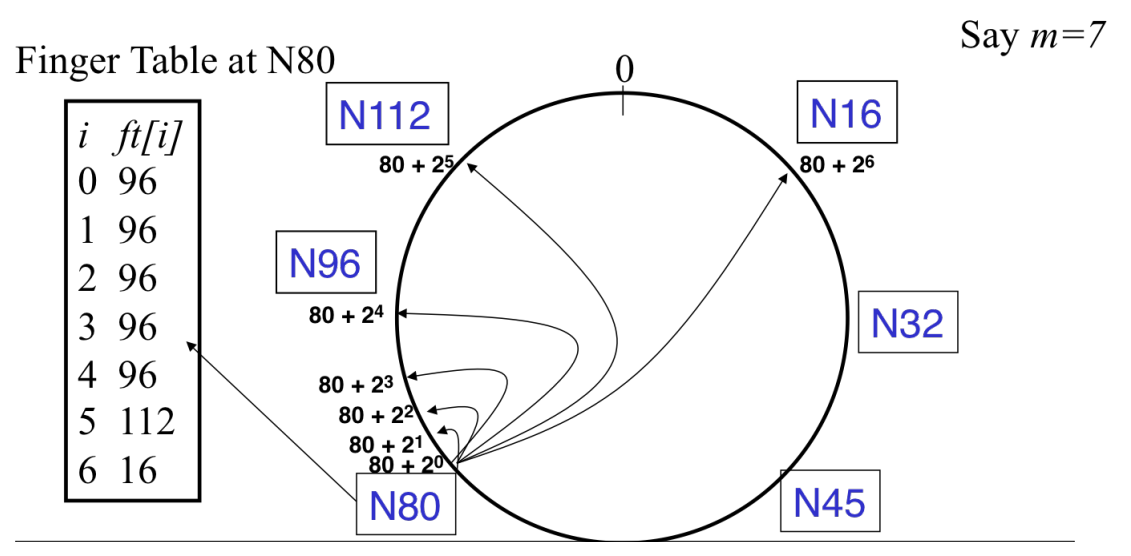
\includegraphics[height=10cm]{chord.png}
    \end{itemize}
\end{frame}

\section{Transport Layer}

\begin{frame}[t]{Transport Layer: Goals}
    \begin{itemize}
        \item We need to provide a \alert{reliable data stream} to the receiver's application from the sender's application. However, there's a lot that can go wrong:
        \begin{itemize}
            \item \pause Packets can be lost
            \item \pause Packets can arrive out-of-order
            \item \pause Packets can be delayed arbitrarily long
            \item \pause Packets can be duplicated
            \item \pause Packets can be corrupted
            \item \pause We can overwhelm a sending/receiving buffer (thereby dropping packets)
            \item \pause If we transmit too much, we can interfere with other communication going on
        \end{itemize}
        \item \pause We don't want to use any information about lower/higher layers
        \item \pause Also, distributed consensus is \textit{hard}. Some of what we want to do is the \alert{Two Generals' Problem}: since message acknowledgments are as likely to be lost as messages, we'd potentially need infinite messages to come to consensus safely.
    \end{itemize}
\end{frame}

\begin{frame}[t]{Transport Layer: Basic Validation}
    \begin{itemize}
        \item Most protocols: to avoid out of sequence ordering, assign each packet a \alert{sequence number}. Send an \alert{acknowledgment} (ACK) if packet received.
        \item \pause Packets can be corrupted. Receiver can calculate \alert{checksum} to verify validity, as well as run ECCs if protocol provides (Hamming codes, etc.) Some protocols send NACKs to indicate that packet has been rejected, but most just ignore packet. 
        \item \pause Idea: Instead of verifying message/ACK reception, have sender simply resend the packet if no ACK has been received after some time. If receiver receives duplicate packet (by sequence number), acknowledge but throw out. \alert{How does this avoid two generals?} \pause Receiver doesn't know (or care) \textit{which} ACKs have been received, so no distributed consensus.
    \end{itemize}
\end{frame}

\begin{frame}[t]{Transport Layer: Pipelined Protocols}
    \begin{itemize}
        \item Validation + one-packet-at-a-time approach is correct, but is intolerably slow. \alert{Solution:} allow \textit{multiple} packets to be ``in-flight'' (forming a \alert{context window})
        \item \pause \alert{Go-Back-$N$} (GBN): Receiver keeps track of the first packet that has \textit{not} been received (expected\_seq\_num). 
        \begin{algorithmic}[1]
        \Procedure{recieve}{$k$}
            \If{$k$ = expected\_seq\_num}
                \State Send ACK($k$); expected\_seq\_num $\gets$ expected\_seq\_num $ + 1$
            \Else
                \State Send ACK(expected\_seq\_num - 1) \Comment{``cumulative ACK''}
            \EndIf
        \EndProcedure
        \end{algorithmic}
        \begin{itemize}
            \item On timeout: resend \textit{all} packets in CW
        \end{itemize}
        \item \pause \alert{Selective ACK}: receiver individually acknowledges all correctly received packets (ACK($k$)), buffers if needed for in-order delivery to application layer. Sender retransmits packets where no ACK received. If receiver receives a packet with the same sequence number as something in the buffer, throw out.
        \item \pause TCP takes a \alert{hybrid approach}, reports cumulative ACKs (lowest seq \# not recieved - 1), but will accept out-of-order packets and reorder them.
        \begin{itemize}
            \item \pause Sender considers multiple ACK($i$)s as \alert{dupACK}s, fresh $i$ in ACK($i$) \alert{newACK}. Useful for estimating congestion.
        \end{itemize}
    \end{itemize}
\end{frame}

\begin{frame}[t]{Transport Layer: TCP Congestion Control}
    \begin{itemize}
        \item \alert{Main Problem}: How large do we make the context window?
        \begin{itemize}
            \item If too large, then router queues fill up, dropped packets, no fair sharing.
            \item If too small, then suboptimal performance.
        \end{itemize}
        \item \pause Initially, (after SYN/SYN-ACK/ACK), transmitter transmits small burst of packets, waits for ACK. Exponentially increases burst size (\alert{slow start}).
        \item \pause After some point (\alert{SST}/\alert{LIT}), switch from doubling the window size every burst to increasing it by 1 per burst.
        \item \pause Sender keeps a timer to interrupt for timeout. When CW shifted, increase the timer by the gap between packets. On timeout, drastically decrease CW, SST, resend packets.
        \item \pause DupACKs aren't necessarily a bad sign, but might be indicator of missed packets. If 3 dupACKs in a row, retransmit DupACK packet but don't reset SST, slightly cut CW (\alert{fast recovery}).
    \end{itemize}
\end{frame}

\begin{frame}[t]{Transport Layer: TCP State Machine}
    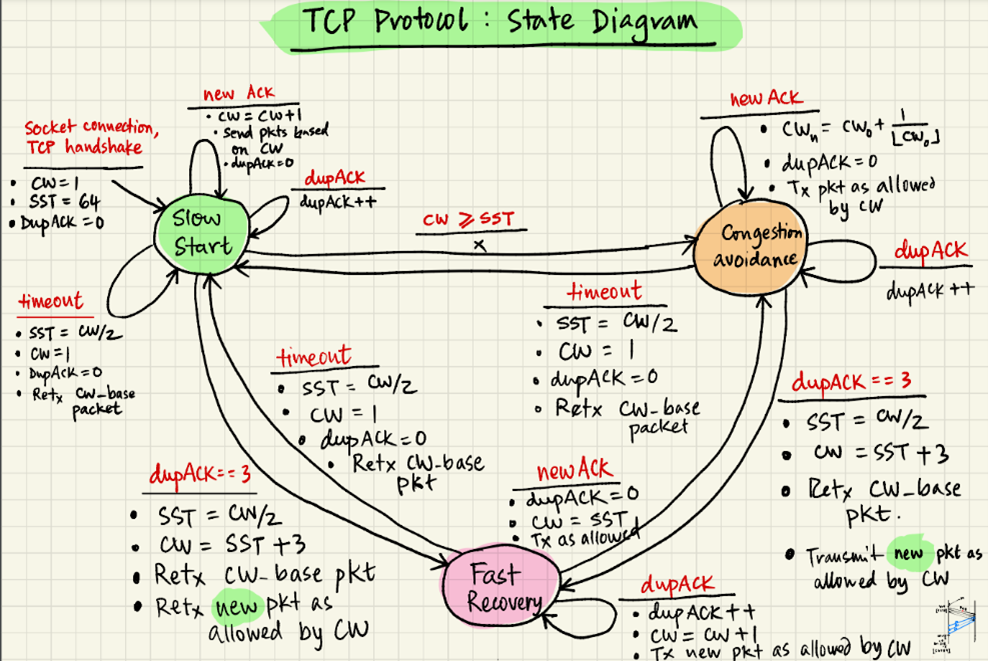
\includegraphics[height=14cm]{tcp flowchart.png}
\end{frame}

\begin{frame}[t]{Transport Layer: TCP RTO Estimation}
    \begin{itemize}
        \item How do we estimate how long timeout (RTO) should be?
        \begin{itemize}
            \item \pause If too short, then premature timeout
            \item If too long, then slow reactions to packet loss
        \end{itemize}
        \item \pause \alert{Intuition}: should be AvgRTT + some ``guard factor''.
        \item \pause AvgRTT estimated by rolling average: $RTT_{avg} \gets (1-\alpha) RTT_{avg} + \alpha\> RTT_{packet}$
        \item \pause ``guard factor'' can be a deviation estimate: \begin{align*}
            devRTT_{avg} &\gets (1-\beta)\> devRTT_{avg} + \beta (|RTT_{packet} - RTT_{avg}|)\\
            RTO &\gets RTT_{avg} + 4\>devRTT_{avg}
        \end{align*}
    \end{itemize}
\end{frame}

\begin{frame}[t]{Transport Layer: Flow Control and Fairness}
    \begin{itemize}
        \item \alert{Problem}: Receiver has a limited buffer. If many nodes transmitting to same receiver, losses may happen at receiver
        \item \pause \alert{Solution}: Receiver reports how much space left to sender in ACKs. Sender will deliberately use a smaller congestion window (while calculating CW as normal).
        \vspace{1cm}
        \item \pause TCP guarantees \alert{max-min fairness} (in stable state): All flows requesting less than fair share get their request. Remaining flows divide equally.
    \end{itemize}
\end{frame}

\section{Network Layer}

\begin{frame}[t]{Network layer (IP)}
    \begin{itemize}
        \item \alert{Goals}: Attempt to send data from one node to another. No guarantees on reliability or anything else.
        \pause\item \alert{Sender}: Recieves data from transport, encapsulated into datagrams, sends it on its way to reciever
        \pause\item \alert{Reciever}: Looks at incoming packets, transmit on to transport layer
        \pause\item \alert{Lots of locality}: the internet is \alert{way} too big for everyone to know how best to send to everyone else, so within a network, our goal is usually just to deliver data to a place where someone else can get it even closer to our destination
        \pause\item Routers examine headers of all IP packets, figure out where to pass it along
    \end{itemize}
\end{frame}

\begin{frame}[t]{Routing vs Forwarding}
    \begin{itemize}
        \item \alert{Routing}: determine the path that packets should take from source to destination (Global)
        \pause\item \alert{Forwarding}: move packets from input buffers to an appropriate output buffer (Local)
        \pause\item Routers run routing algorithms to determine \alert{forwarding table}
    \end{itemize}
\end{frame}


\begin{frame}[t]{Virtual Circuits (potentially skip)}
    \begin{itemize}
        \item Modern networking is \alert{connectionless} (each datagram routed individually) with packets being delivered at \alert{best effort}, but what if we want additional guarantees? We can reserve a \alert{flow/connection} from source to destination, with all packets routed along the flow 
        \pause\item Virtual circuits issued numbers, routers remember which VC number connects to which interface, route all packets coming in with VC to corresponding interface until teardown. \alert{Nothing} else can be sent to that interface.
        \pause\item Steps: (1) Sender initiates call, routers reserve interfaces, (2) receiver accepts incoming call, routers confirm reservation, (3) Sender receives setup confirmation, transmits data, (4) Once transmit done, teardown request sent, reservations released
        \pause\item This sucks (\alert{lots} of residual capacity along links left open), so it's not really used outside of old ATM networks.
    \end{itemize}
\end{frame}

\begin{frame}[t]{Datagram Forwarding (Longest Prefix Matching)}
    \begin{itemize}
        \item Goal: map destination IP to outgoing port
        \pause\item $2^{32}$ possible IP addresses (IPv4), so we can't keep a full table. Instead, map based on \alert{prefix} (i.e. ``All IPs of the form 105.76.x.x should go to interface 5''). \alert{Intuition}: since IPs are hierarchical, nodes with similar IPs are probably pretty close, so the same interface should serve them well
        \pause\item To allow for more finegrained control, allow different prefixes, map packets to \alert{longest} prefix that fully matches (ex: 240.128.x.x/5 is more specific than 128.x.x.x/1, so if both rules in table, choose first)
    \end{itemize}
\end{frame}

\begin{frame}[t]{Routers: The Low-Level View}
    \begin{itemize}
        \item Routers consist of processors (which control routing tables and act in millisecond time frames) and switching fabric (which just simply forwards packets along and acts in nanosecond time frames)
        \item On link-layer receive: using header values, lookup port to send to and queue for transmit. Traditionally, destination-based forwarding (only use destination IP address) is used, but \alert{generalized forwarding} (based on any set of header values) can help at times.
        \item Switching fabric transfers packets between input + output links, goal is to have a high \alert{switching rate} (rate at which inputs -> outputs can be transmit, measured as multiple of input/output line rate). Goal is with $N$ inputs, switching rate of $N$ times line rate
    \end{itemize}
\end{frame}

\begin{frame}[t]{Switching Architectures}
    \begin{itemize}
        \item \alert{Memory}: Have input and output ports on a bus (single use). Load packets into memory, decide where to route, and then send. Super slow, as limited by memory bandwidth; 2 bus crossings per packet.
        \pause\item \alert{Bus}: One wire along which all inputs are connected to all outputs. Faster but still slow, because 1 packet out at a time.
        \pause\item \alert{Others}: Crossbar (only fails when intersection between paths), multistaged switching (switch formed by switches), etc. We can also exploit parallelism by breaking packets up and reassembling them on transmit.
    \end{itemize}
    \begin{center}
        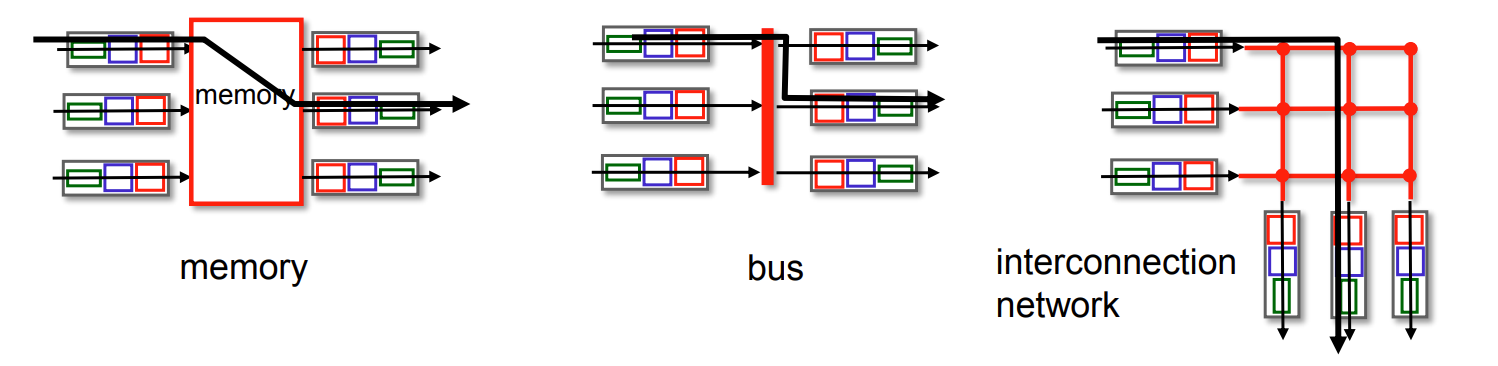
\includegraphics[width = .8\linewidth]{switching arches.png}
    \end{center}
\end{frame}

\begin{frame}[t]{Forwarding and Buffering}
    \begin{itemize}
        \item If switch fabric slower than input ports combined, queues may build up on input. Delay and loss due to buffer overflow possible. 
        \pause\item Problem of \alert{Head-of-the-Line} (HOL) blocking: even if we can send a later packet in our queue, we still have to wait for all earlier packets to be sent!
        \pause\item \alert{Output port queuing}: If datagrams arive from fabric faster than they can be transmit (arrival rate via switching fabric > line speed), then we need a send buffer, and a \alert{drop policy} to decide what to do when we have no space.
        \pause\item \alert{Scheduling discipline} chooses the packets to send first. We can force a priority scheduling scheme to ensure that certain services get best performance and are least affected by high load.
        \pause\item \alert{Buffer Management}: if new packet incoming and buffer full, either tail drop (drop arriving packet) or choose to drop packet on priority basis. 
    \end{itemize}
    
\end{frame}

\begin{frame}[t]{Packet Scheduling}
    \begin{itemize}
        \item How to decide which packet to send on the link next
        \begin{itemize}
            \pause\item \alert{FCFS}: transmit on the order of arrival to output port, can be done using FIFO queue
            \pause\item \alert{Priority scheduling}: Keep separate queues for each priority, transmit from highest priority queue. FCFS within each priority class.
            \pause\item \alert{Round Robin}: have multiple queues, but cyclically switch between classes to send from every time.
            \pause\item \alert{Weighted Fair Queuing}: give each queue a weight, per cycle, spend $\dfrac{w_i}{\sum\limits_j w_j}$ of the cycle on sending from this queue.
        \end{itemize}
    \end{itemize}
\end{frame}


\begin{frame}[t]{IP addressing and Subnets}
    \begin{itemize}
        \item Each network interface (connection between host/router and physical link) given its own IP address (not true in IPv4 anymore but that was the goal)
        \pause\item \alert{Subnets} are a set of devices connected without a router in between, share same IP prefix. Defined by any prefix length using \alert{Classless InterDomain Routing} (CIDR)
        \pause\item Subnet IP designationss of the form a.b.c.d/x where network mask x controls how many bits of prefix to check.
        \pause\item ISPs can seperate a large subnet allocation into a lot of smaller spaces with a wider mask- for example 200.100.16.0/20 can be split into 8 /23 subnets.
        \pause\item IPs can either be allocated \alert{statically} (manually configure on device) or \alert{dynamically} (router assigns to next availiable IP in its subnet), through DCHP
        \begin{itemize}
            \pause\item Client broadcasts request for DCHP server, which issues address. Client confirms use. Can also assign first-hop router, DNS server, network mask.
        \end{itemize}
    \end{itemize}
\end{frame}

\begin{frame}[t]{Network Address Translation (NAT)}
    \begin{itemize}
        \item IPv4 not big enough to fit all of the devices that exist, so let's instead have multiple devices on a subnet share an IP.
        \pause\item Uses transport-layer ports to seperate devices. Routers are given a NAT table to assign (public IP, port) to (private IP, port). 
        \pause\item Routers translate (source, port) to (NAT, NAT port) on outgoing packets, and (NAT, NAT port) to (internal, port) on incoming packets.
        \pause\item Controversial as this breaks layer separation, but extensively used as IPv4 addresses are expensive.
    \end{itemize}
\end{frame}

\begin{frame}[t]{IPv6}
    \begin{itemize}
        \item The ``real'' solution to IPv4 address exhaustion, 128 bit address but fewer additional headers, so 40-byte fixed length
        \item Not every device supports it, so sometimes we need to use IPv4 tunneling: simply encode your IPv6 packet with headers packet as a payload in an IPv4 packet. Set source to the node converting to IPv4, and destination to the node that is back on IPv6.
    \end{itemize}
\end{frame}

\begin{frame}[t]{Routing Protocols}
    \begin{itemize}
        \item \alert{Main Goal}: determine ``good'' paths to send packets from sender to receiver through network of routers
        \pause\item Network can be visualized as a \alert{graph} with nodes being routers and edges being links. Edge weights inversely related to bandwidth, related to congestion, etc. Optimal routing is the \alert{least cost} path.
        \pause\item Algorithms can either be \alert{static} (assume that network costs do not change much, so calculate costs once and leave alone) or \alert{dynamic} (periodically update cost estimates/routes in response to link-cost changes).
        \pause\item Algorithms can either rely on \alert{global} information (all routers have knowledge of network topology, even in areas that are far away) or be built to only use \alert{decentralized} information (routers only know about their own physical connections, and gather everything else from each other)
    \end{itemize}
\end{frame}

\begin{frame}[t]{Link state: Dijkstra's}
    \begin{exampleblock}{Pseudocode}
        \begin{algorithmic}[1]
            \Procedure{LinkState}{$G, s$}
                \State Initialize a table \texttt{distances} to all be $\infty$
                \State Initialize a priority queue \texttt{pq}
                \ForAll{$s \rightarrow t$}
                    \State Add $((s \rightarrow t).\texttt{wt}, t, s)$ to \texttt{pq}
                \EndFor
                \While{\texttt{pq} not empty}
                    \State (dist, node, pred)$\gets\texttt{pq.pop}()$
                    \State Add (dist, node, pred) to \texttt{distances}
                    \ForAll{$\texttt{node} \rightarrow v$}
                        \If{$v$ not in \texttt{distances}}
                            \State Add $(\text{dist} + (\texttt{node} \rightarrow v).\texttt{wt}, v, \text{node})$ to \texttt{pq} (with an \alert{decrease-key} operation if possible)
                        \EndIf
                    \EndFor
                \EndWhile
            \EndProcedure
        \end{algorithmic}
    \end{exampleblock}
    \begin{itemize}
        \pause\item \alert{Upsides}: gives you a full shortest path tree, total runtime fast in comparison to some distance vector algorithms, each node computes its own table so the worst error is a misestimation of link cost.
        \pause\item \alert{Downsides}: needs global information, also oscillations are possible if two paths are nearly equal.
    \end{itemize}
\end{frame}

\begin{frame}[t]{Distance Vector: Bellman-Ford}
    \begin{itemize}
        \begin{exampleblock}{Update Rule}
            $$d(s, t) = \min_{s\rightarrow v}(d(v, t) + (s\rightarrow v).\texttt{wt})$$
        \end{exampleblock}
        \pause \item At each iteration, each node receives updates on connection advertisements from neighbors, then recomputes estimates and advertises new estimates to neighbors
        \pause \item ``Count to infinity'' problem: $A$ can give a lower estimate than expected given a path that uses $A$'s old link cost. Mitigated slightly by ``poisoned reverse'': don't advertise to node $X$ paths that route to node $X$.
        \pause \item Errors propagate through network 
    \end{itemize}
\end{frame}

\begin{frame}[t]{Making Routing Scalable}
    \begin{itemize}
        \item Too many nodes in the internet to calculate full tables
        \pause\item Split up routers into separate \alert{autonomous systems} (UIUC is one)
        \pause\item Intra-AS routing can be chosen by the AS, as long as all routers in AS use same protocol.
        \pause\item \alert{Gateway routers} at the edge of an AS perform inter-domain routing.
        \pause\item Forwarding tables calculated based on domain algorithm for intra-domain routing, both inter-domain and intra-domain for external destinations
        \pause\item Intra-domain protocols/\alert{Interior Gateway Protocols} (IGP) include \alert{RIP} (distance vector), \alert{OSPF} (Link state, with routers flooding entire AS with advertisements with message authentication, multicast, and hierarchical OSPF as ``advanced'' features), and whatever proprietary stuff Cisco does.
    \end{itemize}
\end{frame}

\begin{frame}[t]{Routing between ASes: BGP}
    \begin{itemize}
        \item \alert{eBGP} obtains/shares subnet reachability information with other ASes, \alert{iBGP} propagates internally
        \pause\item eBGP gateways recieve advertisements of routes to other ASes of the form (AS-PATH, NEXT-HOP (specific router in the AS to send requests to)), takes shortest such path known.
        \pause\item Gateways propagate advertisements to internal nodes, other gateways in AS via iBGP, which then advertise to other ASes.
        \pause\item Routers can choose how to send to destination routes based on different criteria including shortest AS-PATH and ``hot potato'' routing (get it out of my AS as quickly as possible)
    \end{itemize}
\end{frame}

\section{Link Layer}

\begin{frame}[t]{Link Layer: Introduction}
    \begin{itemize}
        \item Goal is to transmit a packet over a medium. Each link may have its own protocol.
        \pause\item Encapsulate datagram into \alert{frames}, with \alert{MAC address} used to identify source and destination of hop, provide reliable transmit between the two
        \pause\item Additional services: bit error correction, shared mediums, flow control (your 10Gbps ethernet card will need to send slower so that my 1Gbps ethernet adapter can recieve everything), half (only one of the two sides can transmit at a time) vs full-duplex (both sides can transmit at the same time)
        \pause\item Bit error correction usually done via \alert{pairity checking}: options include single bit, two dimensional pairity checking, Hamming coding, CRC. More reliable transmission mediums will use less complete correction means or will leave it out entirely.
    \end{itemize}
\end{frame}

\begin{frame}[t]{Multiple Access Protocols}
    \begin{itemize}
        \item Often, single shared broadcast channel (unswitched Ethernet, WiFi, etc.). If node receives two or more signals at a time, collision, data wasted, so we need a protocol to determine how we share a channel. Communication about channel sharing must be done via the channel itself. 
        \pause\item Goal is efficient sharing (if only one node wants to transmit, should use full channel rate, otherwise share at $\frac{R}{M}$ if $M$ nodes transmitting), no central server to coordinate, and no synchronization.
        \pause\item Three broad classes:
        \begin{itemize}
            \item \alert{Channel Partition}: Split channel up into smaller ``pieces'': TDMA for time division, FDMA for frequency division
            \pause\item \alert{Random Access}: When node has something to send, send it at full data rate. Protocol detects collisions and how to recover from them. Includes (slotted) ALOHA and CSMA/CD
            \pause\item ``Taking Turns'': Nodes take turns but nodes that have more to send can take longer turns. Includes token-passing (control token giving the right to send passed between nodes)
        \end{itemize}
    \end{itemize}
\end{frame}

\begin{frame}[t]{(Slotted) ALOHA}
    \begin{itemize}
        \item If all frames same size and time divided into equal sized slots, when node receives frame, transmit immediately. If collision, retransmit with probability $p^k$ (with $k$ consecutive failures) for each subsequent frame until success.
        \pause\item If $N$ nodes active, the successful transmit probability is $Np(1-p)$, so for large $N$, successful transmit only happens 37\% of the time!
        \pause\item Unslotted ALOHA doesn't even use slots, synchronization. Performance even worse: 18\% expected success rate.
    \end{itemize}
    
\end{frame}



\begin{frame}[t]{CSMA/CD}
    \begin{itemize}
        \item Listen on channel before transmit. If channel busy, wait until free, then transmit full frame. On collision, abort and choose wait time at random between 0 and $2^m - 1$ for $m$ consecutive collisions
        \item Efficiency trends to 1, so much better than ALOHA
    \end{itemize}
\end{frame}

\begin{frame}[t]{MAC Addressing}
    \begin{itemize}
        \item 48 bit address that's hardcoded, can move between LANs using same address. Each node in a LAN has an (IP address, MAC address, TTL) table. If MAC address not known, node broadcasts ARP query, requested device responds in unicast with its address
        \item Requests outside of LAN are targeted to router, which then will transmit to the outside
    \end{itemize}
\end{frame}

\begin{frame}[t]{Ethernet}
    \begin{itemize}
        \item Topologies include \alert{bus} (all nodes in same collision domain) and \alert{star} (switch in center, no collisions)
        \item Connectionless (no handshaking), unreliable (no acknowledgement), CSMA/CD with binary backoff for MAC
        \item Destination and source MAC addresses, higher layer protocol in header, CRC at end for bit error correction
        \pause\item \alert{Switches} take an active role by selectively forwarding frame to outgoing links, using CSMA/CD to access segment. Hosts are unaware of the presence of switches
        \item Switches are \alert{self learning}: they have a switching table as to what MAC addresses are accessible from which interface. On request coming from node, add its address/interface to table If request designated for known node, send on corresponding interface, else flood.
    \end{itemize}
\end{frame}


\begin{frame}[t]{Wireless}
    \begin{itemize}
        \item A bunch of new considerations that don't exist on wired media: can share frequencies of channel, may want to swap between channnels
        \item Larger issue: signal decay. On wired, you can usually detect all activity over the medium, but on wireless there might be a ``hidden terminal'' that you cannot detect but can interfere with reciever's ability to recieve your message. Also ``exposed terminal'' that you can detect but wouldn't interfere with your transmission because the reciever is out of their range.
        \item Solution: CSMA/CA: Send ``Requests to Send'' (RTS) messages when wanting to send to someone else, wait for ``Clear to Send'' (CTS) from reciever. Nodes only need to not send when they hear a CTS. Still possibility of collisions with data and RTS/CTS packets, but those are much shorter so probability lower.
    \end{itemize}
\end{frame}

\section{Security}
\begin{frame}[t]{Security}
    \begin{itemize}
        \item \alert{Threat Model}: Attacker has access somewhere along the channel that sender and receiver both have. We want to make sure that attacker can't eavesdrop on messages, modify message content, impersonate sender, etc.
        \pause\item More formally, we want to maintain \alert{confidentiality} (only sender and reciever should know what's in the message), \alert{integrity} (no one can modify the message without being detected), and \alert{accessibility} (transmitter should always be able to send to reciever) of data. Also, we want to ensure authentication (receiver should know that transmitter actually sent the data and not someone else).
        \pause\item We'll achieve it through processing data through an \alert{encryption algorithm}. Given some message $m$, we want there to be a $K_e$, $K_d$ s.t. $K_d(K_e(m)) = m$, but it's hard to recover $m$ without some information internal to $K_d$
    \end{itemize}
\end{frame}

\begin{frame}[t]{Symmetric-Key Encryption: AES}
    \begin{itemize}
        \item In a \alert{symmetric-key} scheme, $K_e = K_d$ (or really that $K_e$ and $K_d$ use the same internal information, even if their implementation details are different).
        \pause\item Main implementation is \alert{AES}, which sequentially processes 128 bit ``blocks'' with some incredibly complicated algorithm that is really hard to reverse without knowing the key. Take ECE 407 if you want to know (some of) the details, but \textit{how} it works won't be tested at all. We haven't found a proof that AES is computationally costly to decrypt without a key, but it's survived 20 years of attacks, so we're pretty sure.
        \pause\item Unfortunately, this isn't enough on its own. We don't have a way to transmit decryption keys over an insecure channel (``mailman''/``padlock'' problem), and the keys are shared, so this won't work for authentication.
    \end{itemize}
\end{frame}

\begin{frame}[t]{Public-Key Encryption: RSA}
    \begin{itemize}
        \item Goal is to have two keys $K_-$ and $K_+$, such that $K_+(K_-(m)) = K_-(K_+(m)) = m$. We can obtain $K_+$ from $K_-$ easily, but not the other way. 
        \pause\item Anyone can send publicly undecipherable messages to the private key-holder by encoding them in $K_+$, and the private key holder can send authenticated (but public) messages by encoding them in $K_-$ 
        \pause\item \alert{Main Implementations}: ElGamal, RSA. How RSA works relies on a lot of number theory and the fact that prime factorization is hard. I doubt that questions would be asked on an exam about them (take ECE 407 to learn them). 
        \pause\item Public-key encryption is slow in comparison to symmetric-key encryption, so we often only send AES encryption keys and hashes (one-way function that returns a fixed-length bitstring) of messages under RSA
        \pause\item Still can't tell who someone is unless you know for a fact that their public key is something specific.Have a trusted source (\alert{Certificate Authority}, CA) store this information.
    \end{itemize}
\end{frame}
\section{Practice Questions and Feedback}
\begin{frame}[t]{Practice Questions I}
    \begin{enumerate}
        \item Suppose I implement CDMA/CD, but instead of picking a random pause, I deterministically pause for $2^i$ frames. Will I run into problems if a single machine uses my implementation? What about if many machines are using my implementation on the same ethernet link?
        \pause\item Argue for or against: In a public-key encryption scheme, any message sent that guarantees the authenticity of the sender also guarantees its integrity.
        \pause\item Give an example of a graph with edge costs where there is still a count-to-infinity issue, even with poisoned reverse, after an edge is removed.
        \pause\item I don't want the public internet to know that I'm sending data to a particular port on a machine, so I make a new transport-layer protocol which is exactly the same as UDP but encrypts some fields of transport-layer headers, including the port number using RSA. Is my new transport protocol compatible with the modern internet?
        \pause\item I want to add a link to my network graph that has a negative weight. My AS runs a distance vector protocol. Will this cause problems for the routers? If not, how quickly will distances using my negative link update on other servers?
    \end{enumerate}
\end{frame}
\begin{frame}[t]{Practice Questions II}
    \begin{enumerate}
        \setcounter{enumi}{5}
        \item If an attacker placed a malicious router in a datacenter, could they do more damage if the datacenter was running a distance vector or link-state protocol?
        \pause\item Suppose I have a router with a bus switching fabric that can have packets cross the switching fabric twice as fast as any input port or output port. If I have 3 input ports and 3 output ports, under what load scenarios would I drop packets?
        \pause\item Suppose I have $N$ devices on an wired link using slotted ALOHA that always want to transmit data. Will my link utilization be higher with a lower $N$?
        \pause\item Why do you only need to stop transmission on a channel upon recieving a CTS and not also an RTS?
        \pause\item Explain why a network with a lot of servers but whose activity is mostly transmitting small ``keep alive'' packets would achieve better performance on CSMA/CD over CSMA/CA
        \pause\item If I design a router with a total input capacity equal to the switching speed equal to the total output capacity, do I need to worry about buffers overflowing?
        \pause\item Why do we need IP addresses? Why can't we just route to MAC addresses?
        
    \end{enumerate}
\end{frame}

\begin{frame}[t]{Feedback}
    \begin{center}
        
\includegraphics[height=12cm]{feedback.png}
        http://go.acm.illinois.edu/cs438\_final\_feedback	
    \end{center}
\end{frame}
\end{document}
